\section{Performantie}
\label{sec:evaluatie-performantie}

%%%%%%%%%%%%

Op figuur \ref{fig:performantie} wordt de gemiddelde downloadtijd van de POC en login, zowel niet gecachet als gecachet, voor de vier raamwerken getoond.

\begin{figure}[H]
  \centering
  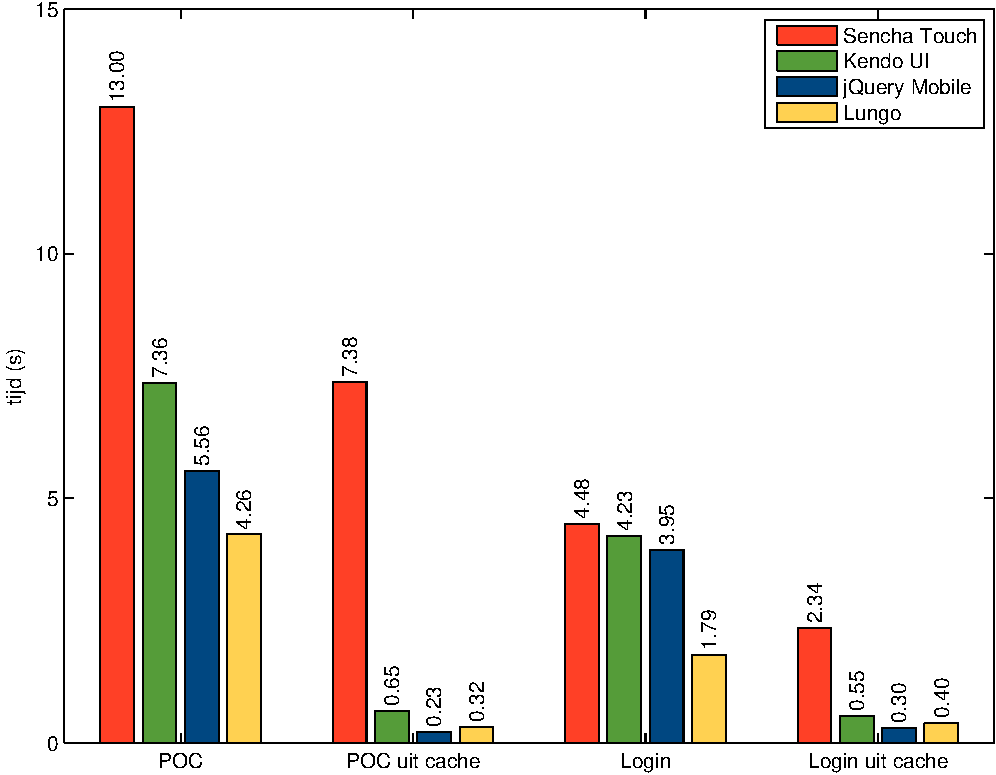
\includegraphics[width=\textwidth]{figuren/performance.pdf}
  \caption{Gemiddelde downloadtijd van POC,  POC uit cache,  login en login uit cache voor elk raamwerk (minder is beter).}
  \label{fig:performantie}
\end{figure}

\lungo{} behaalt de eerste plaats.
Als er gekeken wordt naar de POC heeft \lungo{} maar een derde van de tijd nodig ten opzichte van het traagste raamwerk, \st.
\jqm{} en \kendo{} behalen respectievelijk een tweede en derde plaats.
Aangezien niet alles werd geïmplementeerd in de POC voor \lungo{}, zou men kunnen stellen dat dat de reden is.
Als er echter wordt gekeken naar de loginapplicatie waar alles wel vergelijkbaar is, dan blijft \lungo{} het snelste raamwerk.
Het is zelfs meer dan de helft sneller dan \jqm{}, \kendo{} of \st{}.
Deze drie raamwerken behalen quasi dezelfde opstarttijd, maar ook hier is \st{} terug de traagste.

Als naar de gecachte versie wordt gekeken voor zowel POC als loginapplicatie, scoren \kendo{}, \jqm{} en \lungo{} hetzelfde.
Daarentegen behaalt \st{} telkens een vele tragere tijd.
Enerzijds komt dit doordat de drie eerstgenoemde raamwerken enkel gebruik maken van HTML5 Application Cache.
\st{} gebruikt daarnaast ook nog een eigen mechanisme (zie \ref{sec:performantie-st}) waardoor de grotere laadtijd wordt verklaard.
Anderzijds gebruiken de drie eerstgenoemde raamwerken Yeoman om de applicatie te bouwen.
De webapplicaties gemaakt \st{} gebruiken daarentegen Sencha Cmd.

%%%% De cache factor van ST is constant (gemiddeld 1,8)
%%%% De andere raamwerken hebben een beduidend grotere cache factor 

Indien \st{} buiten beschouwen wordt geladen, duurt het eerste keer laden van de POC gemiddeld 5,73 seconden. Het laden van de gecachete versie duurt slechts gemiddeld 400 milliseconden.
De eerste keer laden van de loginapplicatie duurt gemiddeld 3,32 seconden.
Indien deze werd gecachet, duurt dit nog slechts gemiddeld 420 milliseconden.
Dit zijn aanvaardbare tijden volgens Jakob Nielsen~\cite{Nielsen1993}.
Hij stelt dat indien de tijden onder 1 seconde blijven, de gebruiker de vertraging waarneemt, maar het zijn gedachtengang niet belet.
Tussen de 1 en 10 seconden dient er feedback over het laden te worden gegeven aan de gebruiker.
De browser neemt hiervoor de taak op zich door bij het laden een indicator te tonen.

%TODO: moet Jakob niet worden verplaatst naar het vergelijkingshoofdstuk? 

In wat volgt zullen metrieken worden besproken die de score van de performantie zullen duiden.
De data van de metrieken is weergegeven in tabel~\ref{tabel:performantie-verklaring}.

\paragraph{Google Page Speed}
en eerste extra test is Google Page Speed~\cite{Morgan2011}. 
Deze tool kan de code van een webapplicatie analyseren en testen op performantie specifiek voor mobiele apparaten.
Het resultaat is een score op 100 en een lijst van werkpunten om de performantie van de applicatie te verbeteren.

\paragraph{Gebruikservaring}
Een andere test om de score te toetsen kijkt naar de gebruikservaring.
Hiervoor zal de lijst van $850$ elementen worden gebruikt die getoond wordt na aanmelden op de loginapplicatie.
De auteurs zullen de ervaring bij het scrollen van de lijst vergelijken op de acht apparaten.
De ervaringen per apparaat zullen vervolgens relatief ten opzichte van elkaar beoordeeld worden.

\paragraph{Downloadgrootte en HTML-code}
De HAR-bestanden die werden gebruikt om de laadtijd op te meten bevatten ook de grootte van de pakketten die moeten worden opgehaald.
Omdat pakketten verloren gaan zullen ontvangen bestanden incompleet zijn en moeten ze worden herverzonden. %TODO Sander: klopt dat?
Hierdoor zal het aantal ontvangen bytes variëren van meting tot meting.
De performantietesten werden op acht toestellen uitgevoerd en elke test werd drie keer uitgevoerd.
Het gemiddelde van alle downloadgroottes bepaalt de grootte zoals deze kan worden teruggevonden in tabel~\ref{tabel:performantie-verklaring}.
Bij de POC moet \st{} de meeste data ophalen ($1126.4kB$),  gevolgd door \kendo{} ($194.65kB$), \lungo{} ($249.08kB$) en \jqm{} ($194.65kB$).
Opmerkelijk is dat \lungo{} meer data moet ophalen maar toch een snellere laadtijd behaald.



\begin{table}[H]
\centering
\pgfplotstabletypeset[
  begin table=\begin{tabular}{p{8cm} p{1cm} p{1cm} p{1cm} p{1cm}},
  end table=\end{tabular},
  skip coltypes=true,
  col sep=comma,
  string type,
  header=true,
  columns={Performantie Metrieken,jQM,ST,Kendo,Lungo},
  columns/Performantie/.style={column name=\textbf{Performantie Metrieken}, column type={l}},  
  columns/ST/.style={column name=\textbf{\sta}, column type={c}},
  columns/jQM/.style={column name=\textbf{\jqma}, column type={c}},
  columns/Kendo/.style={column name=\textbf{\kendoa}, column type={c}},
  columns/Lungo/.style={column name=\textbf{\lungoa}, column type={c}},
  every head row/.style={
    before row=\toprule,
    after row=\midrule},
  every last row/.style={
  	before row=\midrule,
    after row=\bottomrule}
]{tabellen/performantie/performantie-verklaring.csv}
\caption{Metrieken gebruikt bij de verklaring van performantiecriterium voor \st{}~(\sta), \kendo{}~(\kendoa), \jqm{}~(\jqma) en \lungo{}~(\lungoa).}
\label{tabel:performantie-verklaring}
\end{table}

% TODO Tim: tabel maken voor de dingen hieronder
% deze dingen uitdiepen hieronder
% page speed
% LOC
% download grootte (POC/login, 1 getal per framework, gemiddelde per device)
% subjectieve experience lijsten
% ST scoort het beste volgens google page speed, maar dat heeft dus te maken met die microlader, daarna volgt lungo, Kendo en jQM die de regels minder strikt, maar uiteindelijk toch sneller presteren

% Sander + LOC uitrekenen
% jQM login<->POC: geen, de beste factor
% ST: immens verschil
% Lungo: zelfde factor als ST
% Kendo de tweede beste factor

% ST was de beste experience, op zowel oude als nieuwe toestellen
% dan volgt jquery mobile, dan lungo en dan kendo
% kendo crashes 
% link naar nelson http://www.nngroup.com/articles/why-you-only-need-to-test-with-5-users/




\subsection{\st}
\label{sec:performantie-st}
% individuele grafiek
% http://www.sencha.com/blog/behind-sencha-command-and-the-build-process
%TODO exacte info tests + extra info CORS zoeken
%TODO AJAX
%Daarnaast zullen geïsoleerde testen met het verzenden van een AJAX-request uitgevoerd worden ($r_{r,AJAX}$).
% Daar wordt het effect van het versturen van een OPTION-\term{request} bekeken wanneer een verzoek naar een ander domeinen wordt gestuurd.


\begin{figure}[H]
  \centering
  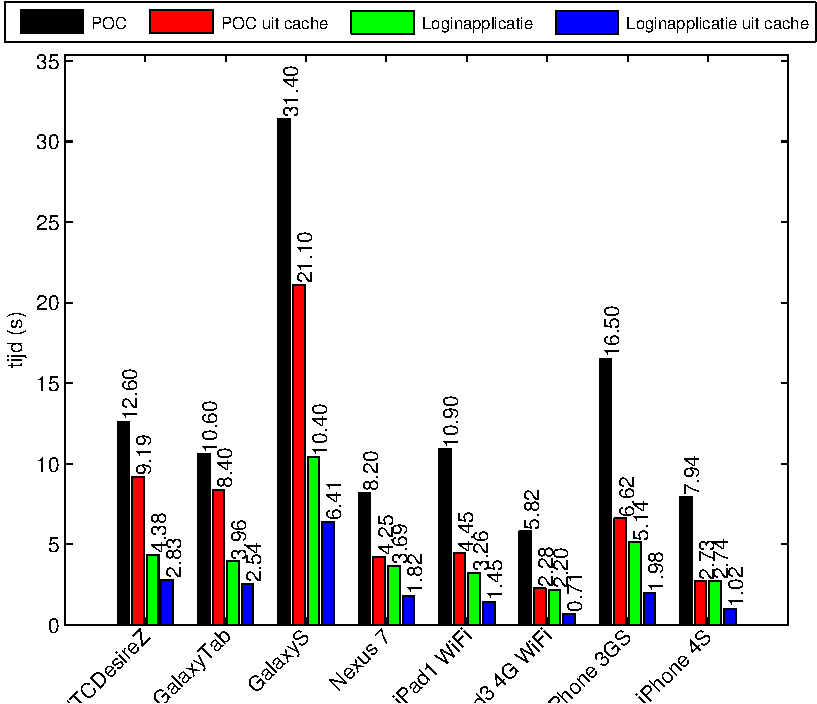
\includegraphics[width=0.5\textwidth]{figuren/performance-st.pdf}
  \caption{Gemiddelde downloadtijden van \st{} voor POC,  POC uit cache,  Login en Login uit cache voor elk apparaat.}
  \label{fig:performantie-st}
\end{figure}

\subsection{\kendo}

\begin{figure}[H]
  \centering
  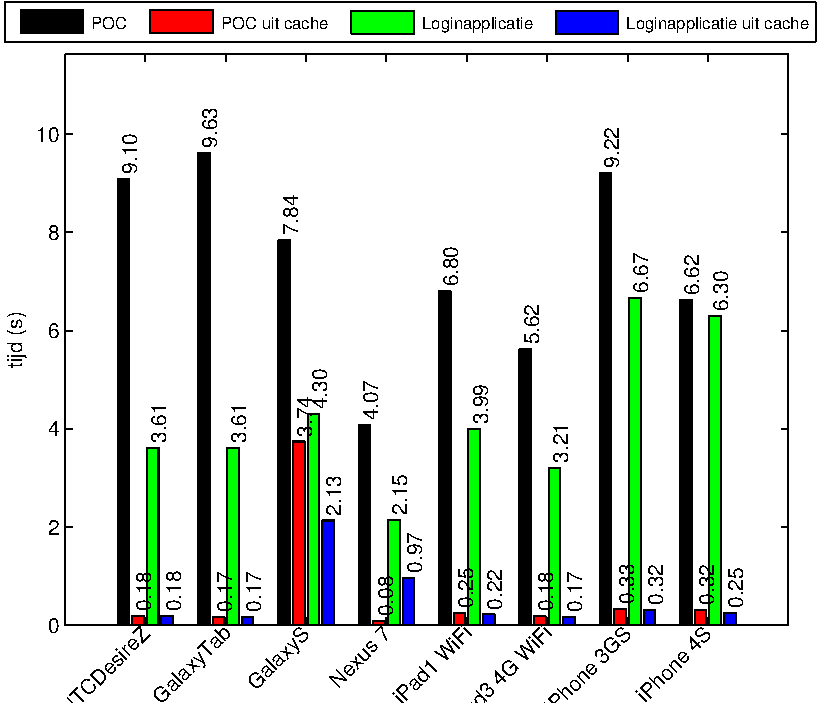
\includegraphics[width=0.5\textwidth]{figuren/performance-kendo.pdf}
  \caption{Gemiddelde downloadtijden van \kendo{} voor POC,  POC uit cache,  login en login uit cache voor elk apparaat.}
  \label{fig:performantie-kendo}
\end{figure}

\subsection{\jqm}
Op figuur~\ref{fig:performantie-jqm} worden de gemiddelde downloadtijd van \jqm{} getoond op elk apparaat.

Voor de POC is een dalende downloadtijd waarneembaar wanneer het Android-apparaat recenter wordt.
Dit is echter ook zo voor de iPads van Apple, maar voor de iPhones stijgt de downloadtijd.
Er zijn minimale verschillen bij de gecachete versie van de POC, waarbij het het langste duurt op de \ipadi{}.

Als de loginapplicatie wordt bekeken, wordt hetzelfde waargenomen als voor de POC.
Enkel bij de Android-apparaten wordt de downloadtijd trager, naarmate het toestel recenter wordt.
Dit is in tegenstelling tot de POC.

Een opmerkelijke waarneming is dat het langer duurt om de gecachete versie van het loginscherm te laden dan de volledige POC.

\begin{figure}[H]
  \centering
  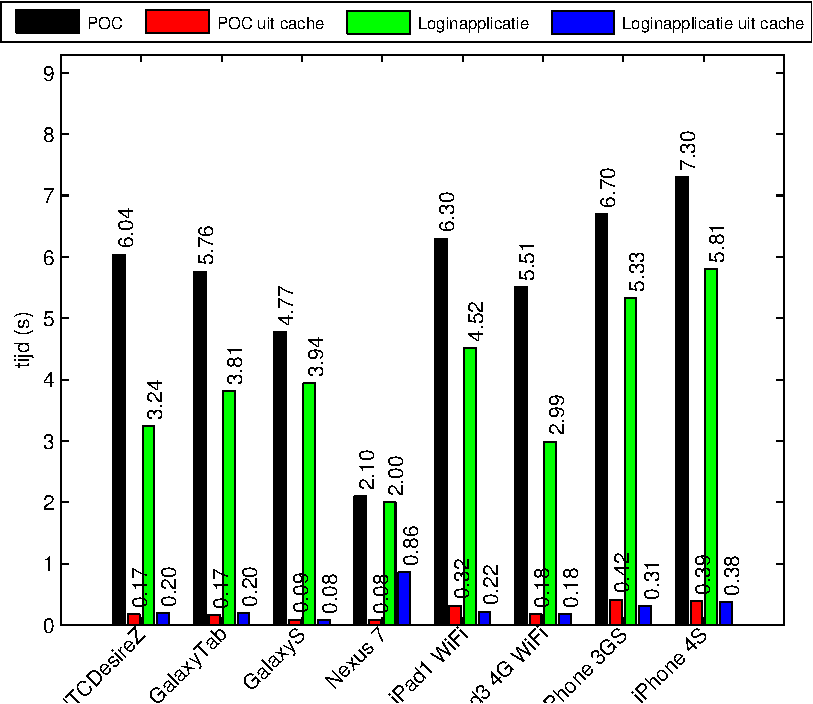
\includegraphics[width=\textwidth]{figuren/performance-jquery.pdf}
  \caption{Gemiddelde downloadtijd van \jqm{} voor POC,  POC uit cache, login en login uit cache voor elk apparaat.}
  \label{fig:performantie-jqm}
\end{figure}

\subsection{\lungo}

\begin{figure}[H]
  \centering
  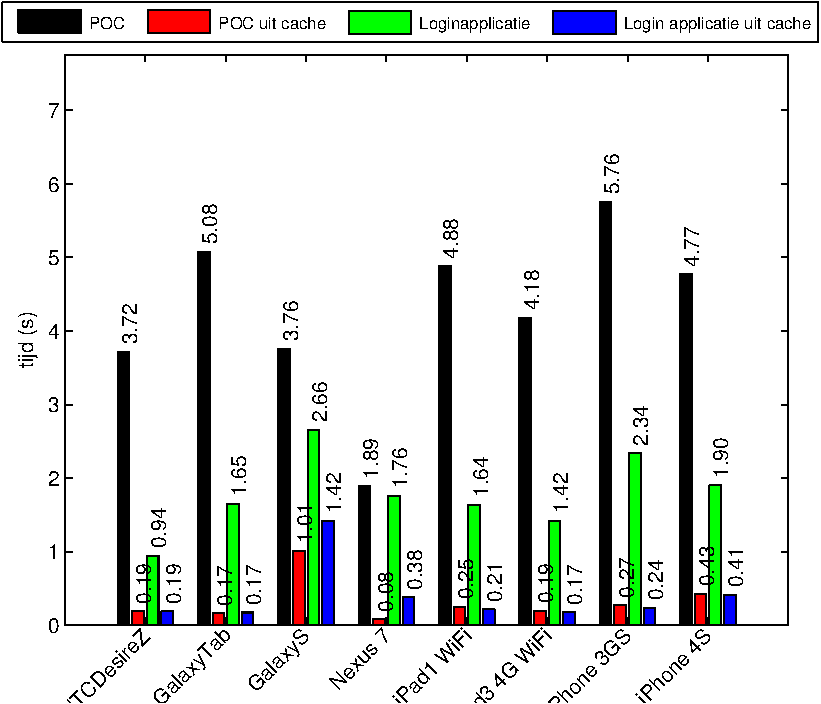
\includegraphics[width=0.5\textwidth]{figuren/performance-lungo.pdf}
  \caption{Gemiddelde downloadtijd van \lungo{} voor POC,  POC uit cache,  Login en Login uit cache voor elk apparaat.}
  \label{fig:performantie-lungo}
\end{figure}
